\section{Distribución $F$}

La distribuci\'on $F$ es fundamental para comparar varianzas y en el an\'alisis de
varianza (ANOVA).

\subsubsection{Definici\'on}

\begin{definicion}[Distribuci\'on $F$]
Sean $\chi^2_{d_1}$ y $\chi^2_{d_2}$ variables chi-cuadrada independientes con
$d_1$ y $d_2$ grados de libertad, respectivamente. La variable aleatoria
\begin{align}
 \label{eq:3.2.15}
 F = \frac{\chi^2_{d_1}/d_1}{\chi^2_{d_2}/d_2}
\end{align}
sigue una distribuci\'on \emph{$F$ de Snedecor} con $(d_1, d_2)$ grados de libertad.
Escribimos $F \sim F_{d_1, d_2}$.
\end{definicion}

{Propiedades}
\begin{itemize}
 \item $F \geq 0$ y la distribuci\'on es asim\'etrica (sesgada a la derecha).
 \item La densidad de $F$ es
 \begin{align}
  \label{eq:3.2.16}
  f(x) = \frac{1}{B(d_1/2, d_2/2)} \left(\frac{d_1}{d_2}\right)^{d_1/2}
  x^{d_1/2 - 1} \left(1 + \frac{d_1}{d_2}x\right)^{-(d_1+d_2)/2},
  \end{align}
  donde $B$ es la funci\'on beta.
 \item $E(F) = d_2/(d_2 - 2)$ para $d_2 > 2$.
 \item $\text{Var}(F) = \dfrac{2 d_2^2 (d_1 + d_2 - 2)}{d_1 (d_2 - 2)^2 (d_2 - 4)}$ para $d_2 > 4$.
 \item Si $F \sim F_{d_1, d_2}$, entonces $1/F \sim F_{d_2, d_1}$.
\end{itemize}

\subsubsection{Aplicaci\'on: comparaci\'on de dos varianzas}

Si $X_1, \ldots, X_{n_1} \sim N(\mu_1, \sigma_1^2)$ y $Y_1, \ldots, Y_{n_2} \sim N(\mu_2, \sigma_2^2)$
son muestras independientes, el cociente de varianzas muestrales
\begin{align}
 \label{eq:3.2.17}
 F = \frac{S_1^2/\sigma_1^2}{S_2^2/\sigma_2^2}
\end{align}
sigue una distribuci\'on $F_{n_1 - 1, n_2 - 1}$ exactamente (por el Teorema de Fisher
aplicado a cada muestra). Bajo la hip\'otesis nula $H_0: \sigma_1^2 = \sigma_2^2$, el
estad\'istico se reduce a $F = S_1^2/S_2^2 \sim F_{n_1-1, n_2-1}$. Esta es la
\emph{prueba $F$ de igualdad de varianzas}.

\begin{teorema}[Intervalo de confianza para $\sigma_1^2/\sigma_2^2$]
 \label{eq:5.5.1}
Con la notaci\'on anterior, un intervalo de confianza del $(1-\alpha)\times 100\%$
para el cociente de varianzas poblacionales es
\begin{align}
 \left[\frac{S_1^2}{S_2^2}\cdot\frac{1}{F_{n_1-1,n_2-1,\,\alpha/2}},\;\;
 \frac{S_1^2}{S_2^2}\cdot F_{n_2-1,n_1-1,\,\alpha/2}\right],
\end{align}
usando la propiedad $1/F_{d_1,d_2} \sim F_{d_2,d_1}$ para expresar el l\'imite
superior con un cuantil de la $F$ ``invertida''.
\end{teorema}

\begin{observacion}[Conexi\'on con la distribuci\'on $t$]
Existe una identidad elegante entre $F$ y $t$: si $T \sim t_\nu$, entonces
$T^2 \sim F_{1,\nu}$. Esto se sigue directamente de las definiciones: $T^2 =
Z^2/(\chi^2_\nu/\nu)$, y $Z^2 \sim \chi^2_1$, as\'i que $T^2$ tiene exactamente la
forma de un cociente de chi-cuadradas escaladas que define a $F_{1,\nu}$. Esta
identidad conecta las tres distribuciones estudiadas en las Secciones
05.03--05.05: $\chi^2$, $t$ y $F$ son, en el fondo, distintas combinaciones de
normales estandarizadas independientes.
\end{observacion}

\subsubsection{Aplicaci\'on: ANOVA}

El an\'alisis de varianza (ANOVA) descompone la variabilidad total de los datos en
componentes atribuibles a distintos factores.

\begin{teorema}[Estad\'istico $F$ en ANOVA]
Consideremos $k$ grupos con $n_i$ observaciones en el grupo $i$-\'esimo, y denotemos
\begin{align}
 \text{SC}_{\text{trat}} &= \sum_{i=1}^k n_i (\bar{X}_i - \bar{X})^2, \\
 \text{SC}_{\text{error}} &= \sum_{i=1}^k \sum_{j=1}^{n_i} (X_{ij} - \bar{X}_i)^2.
\end{align}
Si $H_0: \mu_1 = \cdots = \mu_k$ es verdadera, entonces
\begin{align}
 \label{eq:3.2.18}
 F = \frac{\text{SC}_{\text{trat}}/(k-1)}{\text{SC}_{\text{error}}/(n-k)} \sim F_{k-1, n-k},
\end{align}
donde $n = \sum n_i$.
\end{teorema}

\begin{ejemplo}
 \label{exmp:3.2.6}
Se quiere comparar el rendimiento promedio de tres m\'etodos de ense\~nanza. Se
aplican los tres m\'etodos a grupos de $5$ estudiantes cada uno y se obtienen las
siguientes calificaciones:
\begin{align}
 \text{M\'etodo A: } 85, 90, 78, 92, 88 \quad (\bar{X}_A = 86.6), \\
 \text{M\'etodo B: } 79, 81, 85, 77, 83 \quad (\bar{X}_B = 81.0), \\
 \text{M\'etodo C: } 92, 95, 88, 90, 93 \quad (\bar{X}_C = 91.6).
\end{align}
¿Hay evidencia de que los m\'etodos producen resultados diferentes?
\end{ejemplo}

\begin{solucion}
Calculamos los componentes de varianza:
\begin{align}
 \bar{X} &= \frac{86.6 + 81.0 + 91.6}{3} = 86.4, \\
 \text{SC}_{\text{trat}} &= 5(86.6 - 86.4)^2 + 5(81.0 - 86.4)^2 + 5(91.6 - 86.4)^2 = 290.0, \\
 \text{SC}_{\text{error}} &= \text{var intra-grupo} \times (n - k).
\end{align}
Para simplificar, denotemos los cuadrados dentro de cada grupo. Calculando las
desviaciones de cada observaci\'on respecto a su media de grupo:
\begin{align}
 \text{M\'etodo A: } & (85-86.6)^2 + (90-86.6)^2 + (78-86.6)^2 + (92-86.6)^2 + (88-86.6)^2 = 119.2, \\
 \text{M\'etodo B: } & (79-81)^2 + (81-81)^2 + (85-81)^2 + (77-81)^2 + (83-81)^2 = 40.0, \\
 \text{M\'etodo C: } & (92-91.6)^2 + (95-91.6)^2 + (88-91.6)^2 + (90-91.6)^2 + (93-91.6)^2 = 23.2, \\
 \text{SC}_{\text{error}} &= 119.2 + 40.0 + 23.2 = 182.4.
\end{align}

El estad\'istico $F$ es
\begin{align}
 F = \frac{290.0/(3-1)}{182.4/(15-3)} = \frac{145.0}{15.2} \approx 9.54.
\end{align}

Bajo $H_0$, $F \sim F_{2, 12}$. El valor cr\'itico al $5\%$ es $F_{0.05, 2, 12} = 3.89$.
Como $9.54 > 3.89$, rechazamos $H_0$: hay evidencia de que al menos un m\'etodo
produce resultados diferentes.
\end{solucion}

\lstinputlisting[language=Python]{../code/distribuciones-muestreo/distF.py}

\begin{figure}
 \centering
 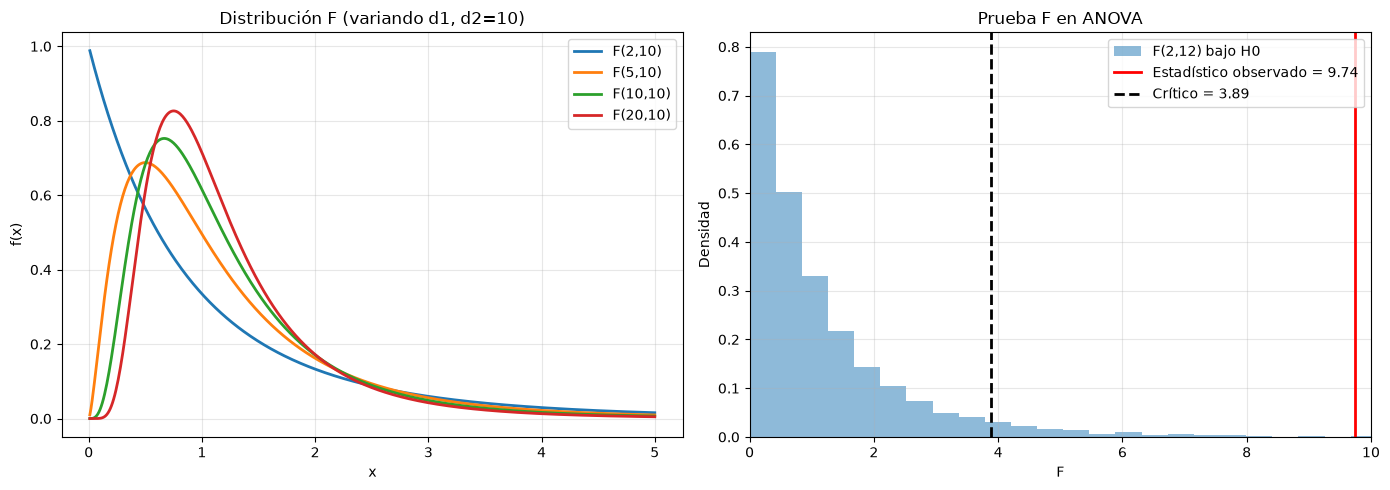
\includegraphics[height=7cm,keepaspectratio=true]{./pe/distF.png}
 % distF.png: 0x0 pixel, 300dpi, 0.00x0.00 cm, bb=
 \caption{Distribuci\'on $F$ de Snedecor y aplicaci\'on al ANOVA.}
 \label{fig:3.2.2}
\end{figure}


